%% ------------------------------------------------------------------
%% clip_examples_subsection.tex
%% A subsection for the Examples section, after the numerical
%% illustration (Section \ref{sec:one-shot:numerical_example}).
%% Figures: fig_oneshot_clip_pca.pdf, fig_labels_capacity.pdf.  Table: clip_auc_table.tex (generated by clip_auc.py).
%% Bib entries: liang2022mind (clip_bib_entries.bib); grechuk2021general exists.
%% ------------------------------------------------------------------

\subsection{One-shot separability of CLIP embeddings}\label{sec:clip-examples}

We return to the embeddings described in the Introduction and compare them with the theory, again for $\alpha=1$. The image embeddings were centred and whitened by principal components, so that the empirical covariance is the identity as in the isotropic setting of Sections~\ref{sec:one-shot:log-concave}--\ref{sec:one-shot:general_log_concave}, and the dependence on dimension was examined by retaining the $n$ leading principal components, ordered by eigenvalue. The label embeddings were treated in the same way for the dependence on dimension; the counts in the full $512$-dimensional space, where whitening would amplify the low-variance directions, use the label embeddings projected onto the unit sphere and centred, which is the geometry in which CLIP uses them. For a set of $N$ points and a map $X\mapsto c(X)$ we estimated $c({\mathbb P}_n,1)$ by the fraction of ordered pairs $(X_i,X_j)$, $j\neq i$, with $(X_j-X_i,c(X_i))\ge0$, over $2{,}500$ random anchors $X_i$ and all $N-1$ other points. Two maps were used: the universal map $c_i=h_1(x_i)$ of (\ref{eq:halpha-def-short}) and the Fisher map $c_i=x_i$; on these data they give indistinguishable results.

{\it The zero-shot rule as a halfspace classifier.} We first quantify the statement made in the Introduction; the numbers are collected in Table~\ref{tab:clip-auc}. On the raw embeddings, without normalisation or centring, the score $(g(z),f(u))$ separates the $100$ images of class $z$ from the $9{,}900$ others with ROC AUC $0.982$ on average over the $100$ classes; $96$ classes exceed $0.95$, and the lowest value, $0.914$, is attained by ``flatfish''. With a threshold $\theta_z$ chosen per class the halfspace $\{x:(g(z),x)\ge\theta_z\}$ captures $95.7\%$ of its own images and $6.4\%$ of the others; the optimal thresholds vary by only $9\%$ across classes, and a single threshold common to all classes loses two points of balanced accuracy. The argmax rule over the $100$ classes gives $72.9\%$ accuracy with raw inner products and $75.8\%$ with cosine similarity. The normal vector $g(z)$ of each halfspace is a proxy for the centroid of the class: after removing the translation common to all classes (the modality gap of \cite{liang2022mind}), the nearest class centroid of every $g(z)$ is the centroid of class $z$ for all $100$ classes in cosine similarity, although the remaining class-specific difference is about half the norm of $g(z)$. The rest of this subsection concerns the question this raises: how many such halfspaces, each built from one representative, can coexist, and how this depends on the dimension.

\begin{table}[tb]
\centering
\begin{tabular}{lccccccc}
\hline
ROC AUC over the 100 classes & min & 10\% & 25\% & median & 75\% & 90\% & max \\
\hline
 & 0.914 & 0.964 & 0.976 & 0.985 & 0.992 & 0.996 & 0.999 \\
\hline
\end{tabular}
\\[2mm]
\begin{tabular}{lccc}
\hline
Halfspace $\{x:(g(z),x)\ge\theta\}$ & balanced accuracy & own images captured & other images captured \\
\hline
threshold $\theta_z$ chosen per class & 0.946 & 95.7\% & 6.4\% \\
one threshold $\theta$ for all classes & 0.927 & 92.7\% & 7.3\% \\
\hline
\end{tabular}
\caption{The zero-shot rule as a halfspace classifier on the raw CLIP embeddings of the CIFAR-100 test set ($10{,}000$ images, $100$ classes). Top: distribution over classes of the ROC AUC of the score $(g(z),f(u))$ for separating the images of class $z$ from all others; the lowest values are ``flatfish'' (0.914), ``man'' (0.934), ``worm'' (0.945), the highest ``bicycle'' (0.999), ``pickup truck'' (0.999), ``sunflower'' (0.999). Bottom: balanced accuracy, recall and false-inclusion rate of the halfspace with the threshold maximising balanced accuracy, chosen per class or common to all classes. The argmax rule over the $100$ classes has accuracy 72.9\% with raw inner products and 75.8\% with cosine similarity.}
\label{tab:clip-auc}
\end{table}


\begin{figure}[tb]
\centering
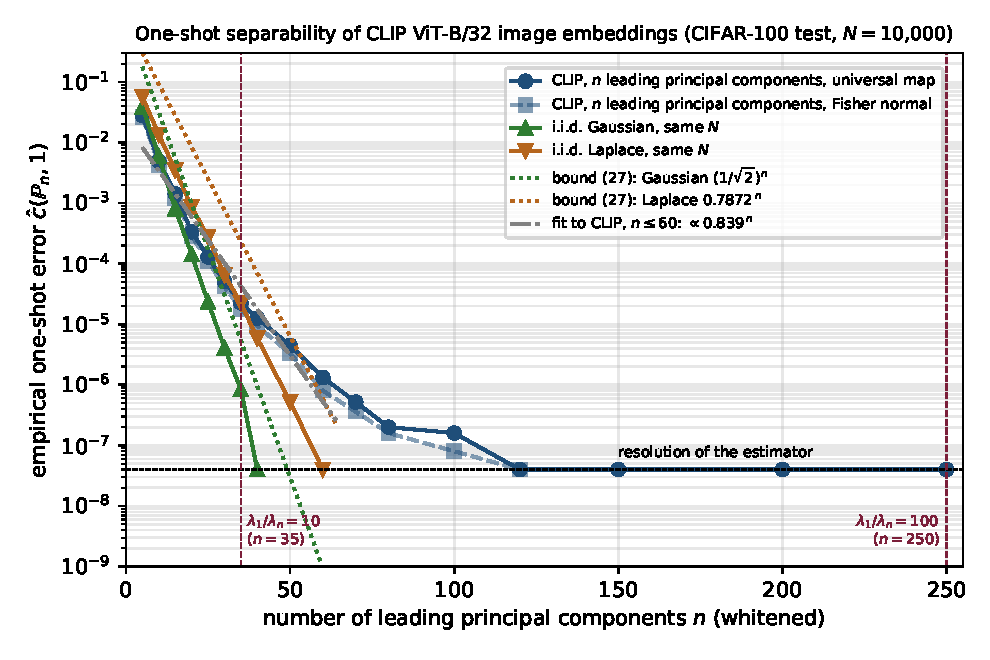
\includegraphics[width=0.7\textwidth]{fig_oneshot_clip_pca.pdf}
\caption{Empirical one-shot separability error $\hat c({\mathbb P}_n,1)$ of CLIP image embeddings (CIFAR-100 test set, $N=10{,}000$) in the subspace of the $n$ leading principal components after whitening, with i.i.d. Gaussian and Laplace samples of the same size, the bounds (\ref{eq:cpnleqcmu}) for these two laws, and a fit $\propto0.839^{\,n}$ to the CLIP data for $n\le60$. The vertical lines mark the dimensions at which the condition number $\lambda_1/\lambda_n$ of the retained components reaches $10$ and $100$; the figure is cut at the latter.}\label{fig:clip-decay}
\end{figure}

{\it Images.} Figure~\ref{fig:clip-decay} shows $\hat c({\mathbb P}_n,1)$ as a function of the number $n$ of leading principal components. For $n\le60$ it decays as $0.839^{\,n}$; in the notation of Table~\ref{tab2} this is $c_{\mathbb P}\approx0.84$ and $b_{\mathbb P}\approx0.09$, slower than the normal ($0.707$) and Laplace ($0.787$) laws and just below the universal constant $C_{hl}(1)<0.85$ of Theorem~\ref{th:logprod}. From $n\approx120$ on, the estimate is at the resolution of the estimator ($4\cdot10^{-8}$, one violating pair), and in the full $512$-dimensional space all $9{,}999$ distinct images are one-shot separable; the two violating ordered pairs there are a duplicated image, i.e. the coincidence of two sample points that no hyperplane can separate (cf. the footnote to Proposition~\ref{prop:oneshot}). The figure is cut at $n=250$, where the condition number $\lambda_1/\lambda_n$ of the retained components reaches $100$; it reaches $10$ already at $n=35$, which is marked for orientation. Beyond these points whitening divides the data by ever smaller eigenvalues ($\lambda_1/\lambda_n\approx750$ at $n=448$, and the last component is degenerate, $\lambda_{512}\approx7\cdot10^{-10}$), so that the whitened trailing coordinates are increasingly dominated by whatever noise the encoder leaves in its low-variance directions; we therefore read the exponent from the well-conditioned range $n\le60$ and regard the counts at larger $n$ only as confirmation that nothing changes when further components are added. Which family of Sections~\ref{sec:one-shot:special}--\ref{sec:one-shot:general_log_concave} does the leading subspace correspond to? Its coordinates are close to log-concave individually (median excess kurtosis $0.6$, log-density concave on $85\%$ of its range), its radius $\|X\|^2/n$ concentrates about as for a Gaussian sample of the same size, and the excess of the rate over the Gaussian one is entirely due to dependence between the coordinates: permuting each coordinate independently, which replaces the distribution by the product of its marginals, brings the rate down to $0.70^{\,n}$. This dependence is directional rather than radial---the leading components carry the cluster structure of the classes, the first of them being bimodal---and a radial model with uniformly distributed directions and the empirical law of the norms underestimates the error (rate $0.67^{\,n}$). In the language of \cite{grechuk2021general}, the embeddings have ``sets of small volume with large probability'', which is precisely what the density ratio in Proposition~\ref{prop:oneshotperturb} controls: the support is bounded, the uniform distribution in a ball is an admissible reference family, and the majorisation constant required to reach the observed rate is of the order $(0.84/0.71)^{\,n}\approx1.2^{\,n}$, within the range $b<1/\sqrt{c_{\mathbb P}}=\sqrt2$ in which the proposition yields exponential one-shot separability. Theorem~\ref{th:logconc}, by contrast, does not apply as stated: the joint distribution is a mixture over classes and is not log-concave.

\begin{figure}[tb]
\centering
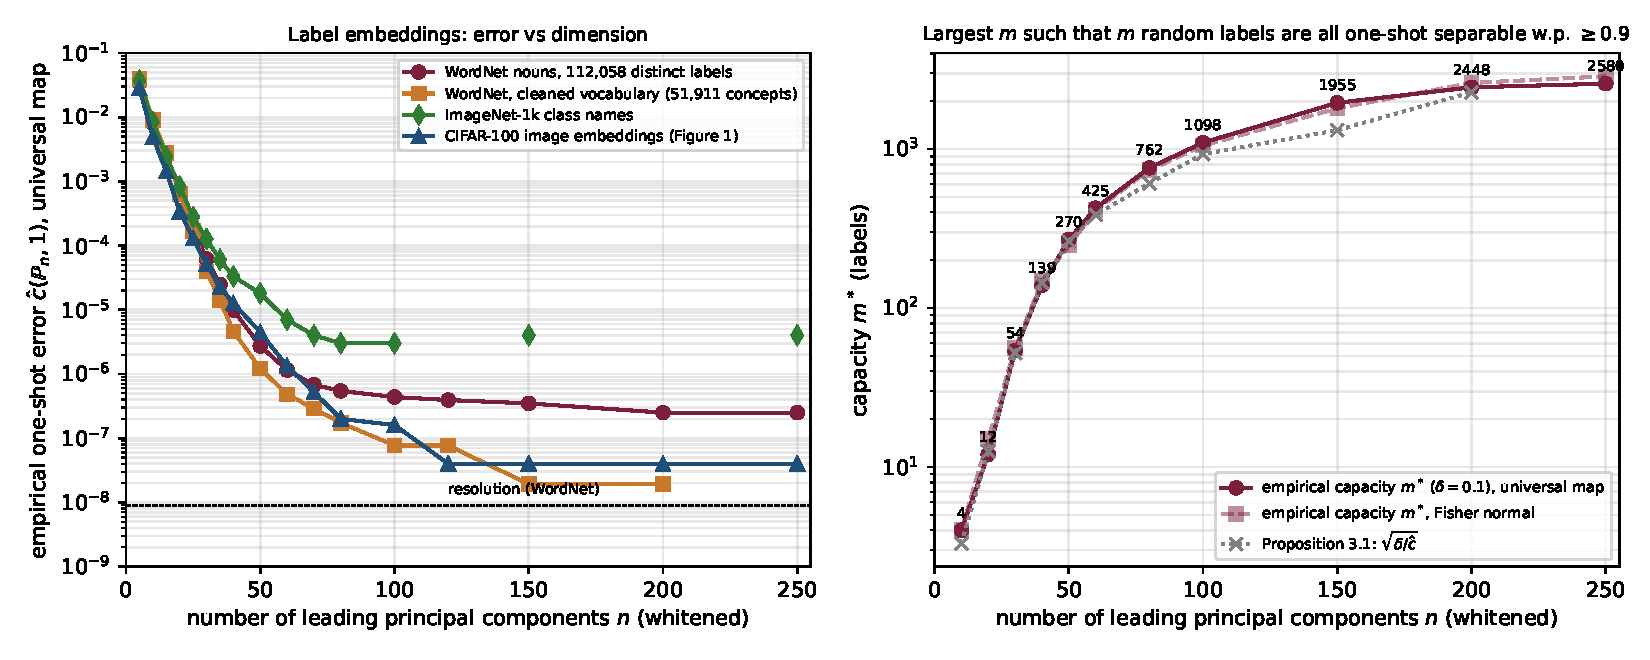
\includegraphics[width=0.98\textwidth]{fig_labels_capacity.pdf}
\caption{Left: $\hat c({\mathbb P}_n,1)$ for the embeddings of the $112{,}058$ distinct WordNet nouns, of the cleaned vocabulary of $51{,}911$ concepts and of the $1{,}000$ ImageNet class names, in the subspace of the $n$ leading whitened principal components, compared with the image embeddings of Figure~\ref{fig:clip-decay}; the label curves level off at the resolution of the estimator or at the level of semantic near-duplicates. Right: the largest $m$ such that $m$ random labels of the cleaned vocabulary are all one-shot separable with probability $0.9$ (universal map and Fisher normal), against the bound $\sqrt{\delta/\hat c}$ of Proposition~\ref{prop:oneshot}.}\label{fig:clip-labels}
\end{figure}

{\it Labels.} For the text embeddings the decay with the number of leading components is at least as fast as for the images up to $n\approx60$ and then levels off (Figure~\ref{fig:clip-labels}, left): for the full WordNet vocabulary at about $3\cdot10^{-7}$, for the ImageNet class names at three violating pairs out of $10^6$, one of which is the class name ``missile'', which occurs twice in the ImageNet label list. What remains at the floor is semantic rather than geometric. In the full space, in the sphere-centred geometry, $1.98\%$ of the WordNet nouns are not separable from some other noun ($3{,}258$ unordered pairs among $112{,}058$ labels); keeping one lemma per WordNet synset reduces this to $1.11\%$, and excluding plant and animal taxa to $0.41\%$, with the universal map and the Fisher normal agreeing to within a few pairs. The remaining inseparable pairs are a term and its modification (``cassette''--``cassette tape'', ``icosahedron''--``regular icosahedron''), a hypernym inside the halfspace of its hyponym (``frog''--``leopard frog''), or ordinal variants (``phase I''--``phase II clinical trial''): the text encoder does not separate what the captions it was trained on did not separate. The capacity of the label space, i.e. the largest $m$ for which $m$ random labels of the cleaned vocabulary are all one-shot separable with probability $0.9$, grows from $4$ at $n=10$ to $54$ at $n=30$, $425$ at $n=60$, $1{,}098$ at $n=100$ and $2{,}580$ at $n=250$ (Figure~\ref{fig:clip-labels}, right). Up to $n\approx60$ it follows the bound $m<\sqrt{\delta/\hat c}$ of Proposition~\ref{prop:oneshot} to within $10\%$, so that on these data the union bound in the proposition is not loose; beyond that the capacity exceeds the bound, because the remaining violations are concentrated on the few labels that have a near-duplicate, whereas the bound treats them as spread over all pairs. Two remarks connect this to the preceding sections. The floor is the coincidence of sample points excluded in Theorem~\ref{thm:lower_bound_one_shot}(a), in a softened form; on the sphere itself, at $\alpha=1$, even near-duplicate labels are separable by the tangent hyperplane, and the floor is a statement about margins, appearing for $\alpha<1$. And the agreement of the capacity with $\sqrt{\delta/\hat c}$ in the well-conditioned range bears on the gap between $m$ and $m^2$ discussed after Theorem~\ref{thm:lower_bound_one_shot}: in the regime of these data the quadratic dependence of Proposition~\ref{prop:oneshot} is the correct one.
